\documentclass{article}
\usepackage[utf8]{inputenc}
\usepackage{hyperref}
\usepackage{amsmath}
\usepackage{amsfonts}
\usepackage{graphicx}


\title{SPhO Ten Year Series (TYS) with Solutions: 2011 Solutions}
\author{
    Solutions available on Victoris\\
    \texttt{victoris.org}
    \and 
    Solutions by Tan Chien Hao\\
    \texttt{www.tchlabs.net}
    % new collaborators add your name and contact here!
}

\date{\today}

\begin{document}
\maketitle


\section{2011}

\subsection{Question 1}
1. A pendulum consists of a copper sphere of radius $R$ and density $\varrho$ suspended from a string. Due to the drag from the air the amplitude of the oscillation $A$ decays with time $t$ as
$$
A=A_{0} \exp (-\gamma t)
$$
where $\gamma=\frac{9 \eta}{4 R^{2} \varrho}$. Ao is the initial amplitude of the pendulum and $\eta$ is the viscosity of air. The measurement of the amplitudes is accurate to $1\%$ with other measurement provided below
$$
\begin{aligned}
	&\eta=(1.78 \pm 0.02) \times 10^{-5} \mathrm{~kg} \mathrm{~m}^{-1} \mathrm{s}^{-1} \\
	&R=5.2 \pm 0.2 \mathrm{~mm} \\
	&\varrho=(0.89 \pm 0.05) \times 10^{3} \mathrm{~kg} \mathrm{~m}^{-3}
\end{aligned}
$$
Evaluate the time taken for the amplitude to fall to $85 \%$ of the initial amplitude $A_{0}$ and the error in this quantity. State the parameter that contributes the biggest error to the final result [8]

\subsection{Solution 1}
\[A=A_0 \exp{(-\gamma t)}\]
Solve for $t$ when $A_0\exp{(-\gamma t)} = 0.85 A_0$
\begin{align}
	t &= -\frac{1}{\gamma} \ln{0.85} \\
	&= -\frac{4R^2\varrho}{9\eta} \ln{0.85} \\
	&= 97.656\text{s}
\end{align}
To find the uncertainty,
\[\frac{\Delta t}{t} = 2\frac{\Delta R}{R} + \frac{\Delta \varrho}{\varrho} + \frac{\Delta \eta}{\eta} + \frac{\Delta \left(\ln\frac{A}{A_0} \right)}{\left|\ln{\frac{A}{A_0}}\right|}\]
To find $\Delta \left(\ln{\frac{A}{A_0}}\right)$ (remembering there is uncertainty in the measurement of $A$ and $A_0$ too),
\begin{align}
	\Delta\left(\ln{\frac{A}{A_0}}\right) &= \Delta(\ln{A} -\ln{A_0}) \\
	&= \frac{\Delta A}{A} + \frac{\Delta A_0}{A_0}
\end{align}
where $\frac{\Delta A}{A} = \frac{\Delta A_0}{A_0} = 0.01$ is given in the question
\begin{align}
	\frac{\Delta R}{R} &= \frac{0.2}{5.2} \\
	\frac{\Delta \varrho}{\varrho} &= \frac{0.05}{0.89} \\
	\frac{\Delta \eta}{\eta} &= \frac{0.02}{1.78} \\
	\frac{\Delta \left(\ln\frac{A}{A_0} \right)}{\left|\ln{\frac{A}{A_0}}\right|} &= \frac{0.01 + 0.01}{ \left| \ln{0.85} \right| }\\
	&= 0.26740 \\
	\Delta t &= 0.26740 \times 97.565 \\
	&= 26 \text{ s (nearest second)} \\
	t &= (98 \pm 26) \text{ s}
\end{align}
Comments: \\
In olympiad it mostly suffices to use the rule \[\Delta f(x_1,x_2,...,x_n) = \left|\frac{\partial f}{\partial x_1}\right| \Delta x_1 + \left|\frac{\partial f}{\partial x_2}\right| \Delta x_2 +...+ \left|\frac{\partial f}{\partial x_n}\right| \Delta x_n \] that looks similar to the multivariate calculus chain rule \[df = \sum_i \frac{\partial f}{\partial x_i} dx_i\]
For example, if $f(a,b,c) = a^2b + c$,
\begin{align}
	\Delta f &= \left| \frac{\partial f}{\partial a} \right| \Delta a + \left| \frac{\partial f}{\partial b} \right| \Delta b + \left| \frac{\partial f }{\partial c} \right| \Delta c  \\
	&= |2ab| \Delta a + |a^2| \Delta b + \Delta c \\
	&= \Delta(a^2 b) + \Delta c\\
	\text{where } \frac{\Delta(a^2 b)}{|a^2 b|} &= \frac{2\Delta a}{|a|} + \frac{\Delta b}{|b|}
\end{align}
The (olympiad) set of rules are then
\begin{align}
	\Delta(A+B) &= \Delta A + \Delta B \\
	\Delta(A-B) &= \Delta A + \Delta B \\
	\frac{\Delta (A\times B)}{|A\times B|} &= \frac{\Delta A}{|A|} + \frac{\Delta B}{|B|} \\
	\frac{\Delta (A\div B)}{|A\div B|} &= \frac{\Delta A}{|A|} + \frac{\Delta B}{|B|}
\end{align}
But in reality, there isn't a hard rule for the calculation of errors and uncertainty. The proper way to do so is using statistics (\url{https://en.wikipedia.org/wiki/Propagation_of_uncertainty}), in which uncertainty is the standard deviation of the distribution of measurements. One commonly used formula is the "quadrature uncertainty".

\subsection{Question 2}
2. In this question you are asked to make reasoned estimates and assumptions. These must be clearly stated.
(a) Figure 1 shows an equilateral glass prism illuminated by a 100 W laser beam of wavelength $\lambda=600$ nm. The refractive index of the glass of the prism is $1.50$ at $\lambda=600 \mathrm{~nm}$. The path of the light in the prism is parelel to the base of the prism. Calculate the change in weight of the prism when the beam is switched on. [4]
\begin{figure}
	\centering
	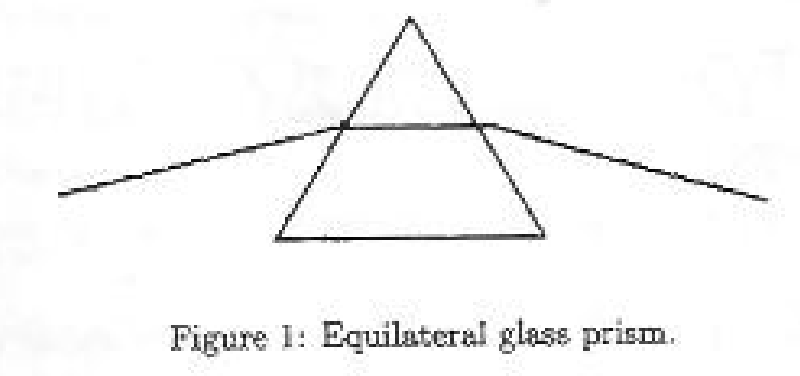
\includegraphics[width=0.8\linewidth]{spho_book_TYS_images/2011q2.png}
	\caption{Equilateral glass prism}
\end{figure}
(b) Optical treezers, which are composed of two lasers beams, are able to manipulate small transparent spheres. Explain clearly how this can be done and why at least two beams are needed. [3]
(c) Small smoke particles in air are seen under a low magnificaton microscope to move randomly at speed of $0.10 \mathrm{~mm}^{-1}$. The speed of sound in air is $20 \mathrm{~m} \mathrm{~s}^{-1}$. Estimate the mass of the smoke particles. [3]

\subsection{Solution 2}
(a) First, find $\theta_i$ by using Snell's law.
\begin{align}
	\sin \theta_i &= 1.5 \sin \theta_r = 0.75 \\
	\theta_i &= 48.590^\circ
\end{align}
Then consider the momentum of one photon before entering the glass and after exiting the glass
\[\Delta p_{vert} = 2p_{photon} \sin{(\theta_i - 30^\circ)} = 2p_{photon} \sin{18.590^\circ}\]
The momentum of a photon is given by the De Broglie wavelength relation (Quantum Mechanics) $p_{photon} = \frac{h}{\lambda}$ where $h$ is Planck's constant and $\lambda$ is the wavelength of the photon. How many photons hit the glass in 1 second?
\[\text{Power} = \frac{\text{Energy}}{\text{Time}} = \frac{hc}{\lambda} \times \frac{\text{No. photons}}{\text{Time}} \]
where $\frac{hc}{\lambda}$ is the energy of one photon. Without explicitly calculating $\frac{h}{\lambda}$, we can now write the force in terms of the power.
\begin{align}
	\text{Force} &= \frac{\Delta p_{vert}}{\text{Time}} \times \text{No. photons} \\
	&= 2\times \frac{\text{Power}}{c} \times \sin(18.590^\circ) \\
	\text{Force} &= 2.1253\times 10^{-7} \text{ N}
\end{align}
Comments:\\
For photon pressure questions, dimensional analysis tends to be useful in guiding your conceptual understanding and checking your formulas.\\
The relativistic energy relation $E^2 = m^2 c^4 + p^2 c^2$ applies to photons as well, where the momentum of a photon is given by the De Broglie relation $\lambda = h/p$\\
For further reading, check out "radiation pressure" and "poynting vector".\\
(b) TODO\\
(c) The speed of sound in a gas is given by \[c=\sqrt{\frac{\gamma P_0}{\rho}}\] where $\gamma$ is the adiabatic constant, $P_0$ is the pressure of the gas, $\rho$ is the density of the gas.
Assuming air to be an ideal gas, $P_0 V = nRT\rightarrow P_0 = \frac{M}{\mu} \frac{RT}{V} = \frac{RT}{\mu} \rho$ where $M$ is the total mass of the gas and $\mu$ is the mass of 1 mole of gas.
Hence, $c=\sqrt{\frac{\gamma RT}{\mu}} $ is the speed of sound.
The speed of sound is related (but not equal!) to the RMS speed $v_{rms}$.
\begin{align}
	\frac{1}{2} n \mu v_{rms}^2 &= \frac{3}{2} nRT\\
	v_{rms} &= \sqrt{\frac{3RT}{\mu}} \\
	&= \sqrt{\frac{3}{\gamma}} \sqrt{\frac{\gamma RT}{\mu}} \\
	&= \sqrt{\frac{3}{\gamma}} c
\end{align}
For air which is around 78\% $\text{N}_2$ and 21\% $\text{O}_2$, let's approximate the no. degrees of freedom to be $f=5$. This gives $\gamma = \frac{f+2}{f} = \frac{7}{5}$.
$v_{rms} = \sqrt{\frac{3}{\gamma}} c = 483.07 \text{ m s}^{-1}$.

\subsection{Question 3}
3. Suppose that we have a string of equally spaced beads of mass m such that their
surfaces are separated by a distance d. The beads are free to slide without friction
on 4 thin wire. Suppose that there is a constant force F acting on the first bead,
initially at rest, and causing it to accelerate along the wire as shown in Figure 2.
This force acts only on the first bead and might be created by a well directed, steady
stream of air. The first bead will collide with the second, which will in turn collide
with the third, and so on. Suppose that all collisions are elastic.

\begin{figure}
	\centering
	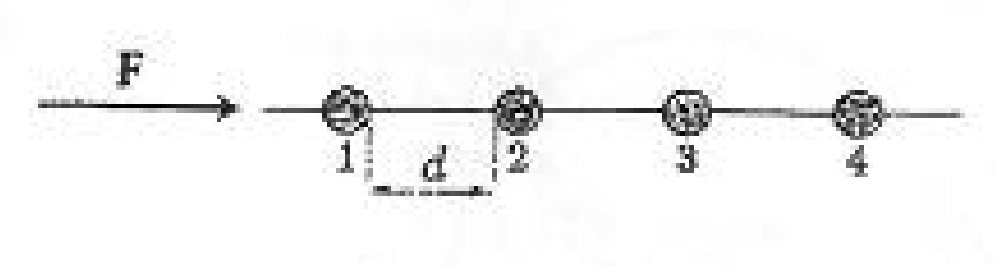
\includegraphics[width=0.7\linewidth]{spho_book_TYS_images/2011q3.png}
	\caption{Beads on wire}
\end{figure}

(i) What is the speed of the first bead immediately before and immediately after its collision with the second bead? [2] \\
(ii) What is the speed of the second bead immediately before and immediately after its collision with the third bead? [2] \\
(iii) Note that the constant force is always acting upon the first bead. What is the time interval between subsequent collisions between the first and second beads? What then is the average speed of the first bead? What is the speed of the “shock wave" that travels down the wire? [3] \\
(iv) If the whole process is repeated, but with collisions which are perfectly inelastic, what is the terminal speed of the shock wave formed? [3] \\

\subsection{Solution 3}
(i) Let the speed of the 1st bead immediately before colliding with the 2nd bead be $v_0$.
\[v_0^2 = 2ad = \frac{2Fd}{m}\]
\[v_0 = \sqrt{\frac{2Fd}{m}}\]
Right after the collision, since the 2nd bead was initially at rest, and has the same mass as the 1st bead, the 1st bead has speed 0 and 2nd bead has speed $v_0$.
(ii) Since the 1st bead does not hit the 2nd bead before the 2nd bead hits the 3rd bead (we will prove this in (iii)),
\begin{align} 
	\text{speed of 2nd bead before collision} &= v_0 \\
	\text{speed of 2nd bead after collision} &= 0
\end{align}
(iii) 
\[\frac{1}{2}\frac{F}{m} t^2 = d\] $t=\frac{2md}{F}$ is the time interval. This answers the first part of (iii). \\
We can now check that the 1st bead does not collide with the 2nd bead before the 2nd bead collides with the 3rd.
\[v_0 t = \sqrt{\frac{2Fd}{m}} \sqrt{\frac{2md}{F}} = 2d > d\]
The 2nd bead would have travelled $2d$ in the time the 1st bead travelled $d$ (to the 3rd bead's starting position). \\
The average speed is then \[v_{ave} = \frac{d}{t} = \frac{d}{\sqrt{\frac{2md}{F}}} = \frac{Fd}{2m} = \frac{1}{2} v_0\]
The speed of the shockwave is just $v_0$. You may think of the speed of the shockwave as the collissions and how they move down the chain. Each successive collission is distance $d$ apart and takes time $d/v_0$ seconds. Hence the speed is just $d/(d/v_0) = v_0$.
(iv) We solve this with various methods. \\
Method 1: \\ 
This is an exact method but it requires numerical calculation which is not available during the competition. Method 2 would be preferred during the competition.
Let $v_n$ be the velocity of the lump of mass $m$. By conservation of momentum,
Before: insert diagram
After: insert diagram
\begin{align}
	(n+1) m v_n' &= nm v_n\\
	\rightarrow	v_n' &= \frac{n}{n+1} v_n
\end{align}
The $(n+1)m$ mass then undergoes acceleration caused by force $F$ until the moment right before it collides with the $(n+2)$-th mass.
\[v_{n_1}^2 = v_n'^2 + 2 \frac{F}{(n+1)m} d = \frac{n^2}{(n+1)^2} v_n^2 + 2\frac{F}{(n+1)m} d \]
\[v_{n+1} = \sqrt{\frac{n^2 v_n^2}{(n+1)^2} + \frac{2Fd}{(n+1)m}}\]
Numerically, one can solve this recurrence relation to obtain $v_n \rightarrow \sqrt{\frac{Fd}{m}}$, which is the terminal velocity.\\
I still don't know how to solve this without resorting to numerical methods like Mathematica. However, method 2 is completely doable in a competition setting.

Method 2: \\
This method is not 100\% precise, but it replaces the discrete problem with a continuous one. \\
Let $M$ be the mass of the collected beads.
\begin{align}
	F &= \frac{d}{dt} (Mv) \\
	&= \frac{dM}{dt} v + M \frac{dv}{dt}
\end{align}
Since $\frac{dv}{dt} = 0$ at terminal velocity,
\begin{align}
	F &= \frac{dM}{dt} v \\
	&= \frac{dM}{ds} \frac{ds}{dt} v \quad \text{where } s \text{ is the displacement of the collected beads}\\
	&= \frac{m}{d} v^2 \quad \text{ since }\quad \left(\frac{dM}{ds} = \frac{m}{d}\right)\\
	v &= \sqrt{\frac{Fd}{m}}
\end{align}
And we are done!

\subsection{Question 4}
4. A zoom lens system is a combination of lenses that produces a variable magnification while maintaining fixed object and image positions. The magnification is varied by moving one or more lenses along the axis. While multiple lenses are used in practice to obtain high-quality images, the effect of zooming in on an object can be demonstrated with a simple two-lens system. An object, two converging lenses, and a screen are mounted on an optical bench. The first lens, which is to the right of the object, has a focal length of 5.0 cm, and the second lens, which is to the right of the first lens, has a focal length of 10.0 cm. The screen is to the right of the second lens. Initially, an object is situated at a distance of 7.50 cm to the left of the first lens, and the image formed on the screen has a magnification of 1.00. \\
\\
(i) Determine the distance between the object and the screen. [4] \\
(ii) Both lenses are now moved along their common axis, while the object and the screen maintain fixed positions, until the image formed on the screen has - magnification of $+3.00$. Find the displacement of each lens from its initial position in (i). [4] \\
(iii) Can the lenses be displaced in more than one way? [4] \\

\subsection{Solution 4}
(i) Concept: When looking at multiple lens systems, we simply treat the image formed by one lens as the object for the next lens. Convince yourself by considering where all possible light rays pass through after the first lens. \\
insert diagram \\
Namely, it is important to note that this approach assumes the radius of the lens is infinite. It is worth considering cases where the lens has finite radius, which will produce a "trimmed image". While these type of questions have not appeared in SPhO, they have appeared n other competitions like EuPhO 2020 Q3. \\
Anyway, returning to the question, (i) is just a direct application of this "multiple lens" concept with simple algebraic manipulation.\\
insert diagram
\[f_1 = 5.00 \text{ cm}\]
\[f_2 = 10.00 \text{ cm}\]
\[x_0 = 7.50 \text{ cm}\]
\[M = \frac{y}{x-x_1} \frac{x_1}{x_0} = 1.00\]
\[\frac{1}{x_0} + \frac{1}{x_1} = \frac{1}{f_1}\]
\[x_1 = \frac{x_0 f_1}{x_0 - f_1} = 15.0 \text{ cm}\]
\[\frac{y}{x-x_1} \frac{x_1}{x_0} = 1\]
\[y=\frac{x_0}{x_1} (x-x_1) \Rightarrow \frac{1}{y} = \frac{x_1}{x_0(x-x_1)}\]
\[\frac{1}{f_2} = \frac{1}{x-x_1} + \frac{1}{y}\]
\[ \frac{1}{f_2} = \frac{1}{x-x_1} + \frac{x_1}{x_0} \frac{1}{x-x_1} \]
\[ x - x_1 = \left(1+\frac{x_1}{x_0}\right) f_2 \]
\[x = \left(1+\frac{x_1}{x_0}\right) f_2 + x_1=45.0\text{ cm}\]
\[y = \frac{x_0}{x_1} (x-x_1) = 15.0\text{ cm}\]
The distance between the object and the screen is $L=x_0+x+y=67.5\text{ cm}$.

$$
\begin{array}{l}
	x_{0}+x+y=L=67.5 \mathrm{~cm} . \\
	\frac{y}{x-x_{1}} \cdot \frac{x_{1}}{x_{0}}=M=3 \\
	\frac{1}{x_{0}}+\frac{1}{x_{1}}=\frac{1}{f_{1}}=\frac{1}{5 \cdot 00 \mathrm{~cm}} \\
	\frac{1}{x-x_{1}}+\frac{1}{y}=\frac{1}{f_{2}}=\frac{1}{10.0 \mathrm{~mm}}
\end{array}
$$
One way to solve this is to use Eq $2,3,4$ to get expressiens of $y$ and $x$ in tems of $x_{0}$, whish we $\mathrm{~ c a n ~ t h e y ~ s m b r i t h e ~ b a c k}$ Unfertunately, the follewhe calculanens are vey tedious and requhe great cane.
From (2), $\frac{1}{x-x_{1}}=\frac{m_{x_{0}}}{y x_{1}}$
Subsititning thass ihto (4),
$$
\frac{1}{y}\left(\frac{m x_{0}}{x_{1}}+1\right)=\frac{1}{f_{2}}
$$
Sulkslituthy (3) thto the above,
$$
\begin{array}{l}
	\frac{1}{y}\left(M_{x_{0}}\left(\frac{1}{f_{1}}-\frac{1}{x_{0}}\right)+1\right)=\frac{1}{f_{2}} \\
	y=f_{2}\left(\frac{m_{x_{0}}}{8_{1}}-M+1\right)
\end{array}
$$

\subsection{Question 5}

(i) A stick of mass density per unit length $\rho$ rests on a circle of radius $R$ (see Figure 3). The stick makes an angle $\theta$ with the horizontal and is tangent to the circle at its upper end. Friction exists at all points of contact, and assume that it is large enough to keep the system at rest. Find the friction force between the ground and the circle. [6]

\begin{figure}
	\centering
	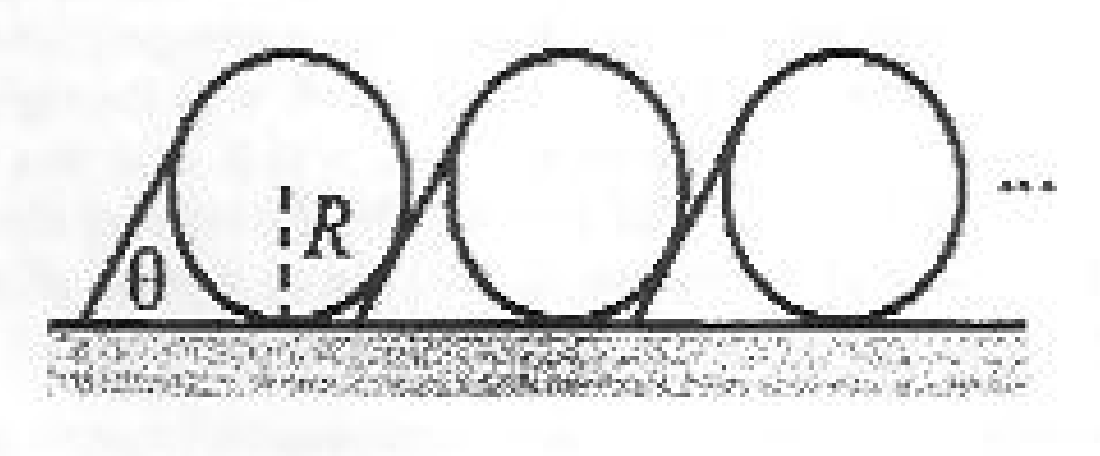
\includegraphics[width=0.7\linewidth]{spho_book_TYS_images/2011q5.png}
	\caption{Stick on a circle}
\end{figure}
(2) A large number of sticks (with mass density per unit length $\rho$) and circles (with radius $R$) lean on each other, an shown in the Figure below. Each stick makes an angle $\theta$ with the horizontal and is tangent to a circle at its upper end. The sticks are hinged to the ground, and every other surface is frictionless unlike in the first part of this question in (i)]. In the limit of a very large number of sticks and circles, what is the normal force between a stick and the circle it rests on very far to the right? (Assume that the last circle leans against a wall, to keep it from moving) [6]


\subsection{Solution 5}
Q4(ii) Referring to the same diagram, we are aive allomed fo vary $x_{0}, x, y$ such that they satisfy 4 anneradht guotars,

From (2),
$$
\begin{array}{l}
	x-x_{1}=\frac{y_{1}}{m_{00}} \\
	x=\left(\frac{y}{m x_{0}}+1\right) x_{1} \\
	\quad=\left(\frac{f_{2}\left(\frac{m x_{0}}{f_{1}}-M+1\right)}{m_{x_{0}}}+1\right) x_{1}
\end{array}
$$$$
n-+h \text { ball }
$$ ball and surdes or lall and Aloor,
$$
N_{n}=N_{n}^{\prime}
$$
Ther conside fle $(n+1)$ th stick.
consille torque abent the hinge,
$$
\begin{array}{l}
	N_{n+1} l=\frac{m g l}{2} \cos \theta-N_{n} R \tan \frac{\theta}{2}=0 \\
	\text { Whth } l=\frac{R}{\tan \frac{\theta}{2} .} \\
	\frac{N_{n+1} R}{\tan \frac{\theta}{2}}-\frac{m g R}{2 \tan \theta} \cos \theta-N_{n} R \tan \frac{\theta}{2}=0 . \\
	N_{n+1}=N_{n} \tan ^{2} \frac{\theta}{2}+\frac{m g}{2} \cos \theta
\end{array}
\begin{aligned}
	N_{n} &=N_{n-1} \tan ^{2} \frac{\theta}{2}+\frac{m g}{2} \operatorname{as} \theta \\
	&=\left(N_{n-2} \tan ^{2} \frac{\theta}{2}+\frac{m}{2} \cos \theta\right) \tan ^{2} \theta_{2}+\frac{m g}{2} \cos \theta \\
	&=N_{n-2}\left(\tan ^{2} \frac{\theta}{2}\right)^{2}+\frac{m g}{2} \operatorname{as} \theta\left(1+\tan ^{2} \frac{\theta}{2}\right) \\
	&\left.=N_{n-3}\left(\tan ^{2} \frac{\theta}{2}\right)^{3}+\frac{m g \cos \theta\left(1+\tan ^{2} \theta+\tan \frac{4 \theta}{2}\right)}{2}\right) \\
	&=N_{n-4}\left(\tan ^{2} \frac{\theta}{2}\right)^{4}+\frac{m g}{2} \cos \theta\left(1+\tan ^{2} \frac{\theta}{2}+\tan ^{4} \frac{\theta}{2}+\tan ^{6} \frac{\theta}{2}\right) \\
	&=\cdots \\
	&=N_{0}\left(\tan ^{2} \frac{\theta}{2}\right)^{n}+\frac{m g}{2} \operatorname{as} \theta\left(\frac{1-\tan ^{2 n} \frac{\theta}{2}}{1-\tan ^{2} \frac{\theta}{2}}\right)
\end{aligned}
$$
A, $n \rightarrow \infty, \quad\left(\tan ^{2} \frac{\theta}{2}\right)^{n} \rightarrow 0 \quad$ because $\theta<\pi / 2$
$\lim _{n \rightarrow \infty} N_{n}=\frac{m g}{2} \frac{\operatorname{asc} \theta}{1-\tan ^{2} \frac{\theta}{2}}$
$=\frac{\rho R g}{2} \frac{\cos \theta}{\left(1-\tan ^{2} \frac{\theta}{2}\right) \tan \frac{\theta}{2}}$
$=\frac{\sin g}{2} \frac{\cos \theta \cos ^{2} \frac{\theta}{2}}{\left(\cos ^{2} \frac{\theta}{2}-\sin ^{2} \frac{\theta}{2}\right) \tan \frac{\theta}{2}}$
$=\frac{\rho^{2 g}}{2} \cos ^{2} \frac{\theta}{2} \cot \frac{\theta}{2}$




\subsection{Question 6}
6. An aluminum rod $0.500 \mathrm{~m}$ in length and with a cross-sectional area of $2.50 \mathrm{~cm}^{2}$ is inserted into a thermally insulated vessel containing laguid helinm at $4.20 \mathrm{~K}$. The rod is initidy at $300 \mathrm{~K}$. \\
(i) If half of the rod is inserted into the helium, how many liters of helium boil off by the time the inserted half cools to $4.20 \mathrm{~K} ?$ (Assume the upper half does not yet cool.) [4] \\
(ii) If the upper end of the rod is maintained at $300 \mathrm{~K}$, what is the approximate boil-off rate of liquid helium after the lower half has reached $4.2 \mathrm{~K} ?$ (Aluminum has thermal conductivity of $31.0 \mathrm{~J} \mathrm{~s}^{-1} \mathrm{~cm}^{-1} \mathrm{~K}^{-1}$ at $4.2 \mathrm{~K}$ You may ignore its temperature variation. Note that aluminum has a specific heat capacity of $902 \mathrm{~J~kg}^{-1} \mathrm{~K}^{-1}$ and density of $2700 \mathrm{~kg} \mathrm{~m}^{-3}$. The density of liquid helium is $125 \mathrm{~kg} \mathrm{~m}^{-3}$.) [4] \\


\subsection{Solution 6}


\subsection{Question 7}

7. A soap film $(n=1.33)$ is contained within a rectangular wire frame. The frame is held vertically so that the film drains downward and forms a wedge with flat faces. The thickness of the film at the top is essentially zero. The film is viewed in reflected white light with near-normal incidence, and the first violet (the wavelength is 420 nm) interference band is obsarved $3.00$ cm from the top edge of the film. \\
(j) Locate the first red $(\lambda=600 \mathrm{~nm})$ interference band. [4] \\
(ii) Determine the film thickness at the positions of the violet and red bands. [3] \\
(ii) What is the wedge angle of the film? [3] \\

\subsection{Solution 7}

\subsection{Question 8}

8. A solenoid of length $2 \ell$ has an inner radius $R_{1}$ and arrouter radius $R_{2}$. The current through the solenoid is $I$. \\
(i) Show that the magnetic flox density, $E$ at the center of the solenoid is
$$
B=\kappa n I \ell \frac{\alpha+\left(\alpha^{2}+\beta^{2}\right)^{1 / 2}}{1+\left(1+\beta^{2}\right)^{1 / 2}}
$$
where $n$ is the number of turns per square meter and $\alpha$ and $\beta$ are functions of $R_{1}, R_{2}$ and $L$. Write down the exprestion for $\alpha$ and $\beta$. State the value of $\kappa$. \\
(ii) Show that the length of the wire is
$$
\ell=n V=2 \pi n\left(\alpha^{m_{1}}-1\right) \beta^{m_{1}} R_{1}^{m_{2}}
$$
where $V$ is the volume of the winding and $m_{1}, m_{2}$ and $m_{3}$ are exponents thet need to be determined. State the value of $m_{1}, m_{2}$ and $m_{3}$. \\
(iii) Show that the $B$ field at the center of the solenoid can be written as
$$
B=G\left(\frac{P \lambda \sigma}{R_{1}}\right)^{1 / 2}
$$
where $G$ depends on the geometry, $P$ is the dissipated power, $\lambda=\pi \pi r^{2}$ is the filling factor or fraction of the coil cross sechon oocupied by the conductor, $r$ is the radius of the wire and $\sigma$ is the conductivity. [4]

\subsection{Solution 8}

\subsection{Question 9}
9. (a) A large block, with a second block sitting on top, is connected to a spring and executes horizontal simple harmonic motion as it slides across a frictionless surface with an angular frequency $\omega$. The coefficient of static friction between the two blocks is $\mu_{s}$. Derive a formula for the maximum amplitude of oscillation that the system can have if the upper block is not to slip. (Assume that the mass of the spring is negligible.) [6] \\
(b) A pencil of length $L_{1}$ with the pencil point at one end and an eraser at the other end, is initially standing vertically on a table with the pencil point on the table. The pencil is let go and falls over. Derive a formula for the speed with which the craser strikes the table, assuming that the pencil point does not move. [4]

\subsection{Solution 9}

\subsection{Question 10}
10. (a) The Oscillation Project with Emulsion-tRacking Apparatus (OPERA), an experiment designed to test neutrino ostillations and exploiting the high energy muon neutrino produced at CERN Super Proton Synchrotron in Geneva and pointing towards Gran Sasso in Italy, reported that the time of flight messurements indicated that muon neutrinos trave! at speed $v$ which is faster than the speed of light with $\beta=\frac{v}{c}=1+1.48 \times 10^{-5}$, where $c$ is the speed of light in vacua. Show that it is possible for an observer moving relative to the Earth starting at CERN and moving towards Gran Sasso at some critical speed $u$ to see the muon neatrino moving backwards from Gran Sasso towards CERN and determine this critical speed.\\
(b) A moving rod is observed to have a length of $2.00 \mathrm{~m}$ and to be oriented at an angle of $30.0^\circ$ with respect to the direction of motion, as shown in the Figure below. The rod has a speed of $0.995~c$.
\begin{figure}
	\centering
	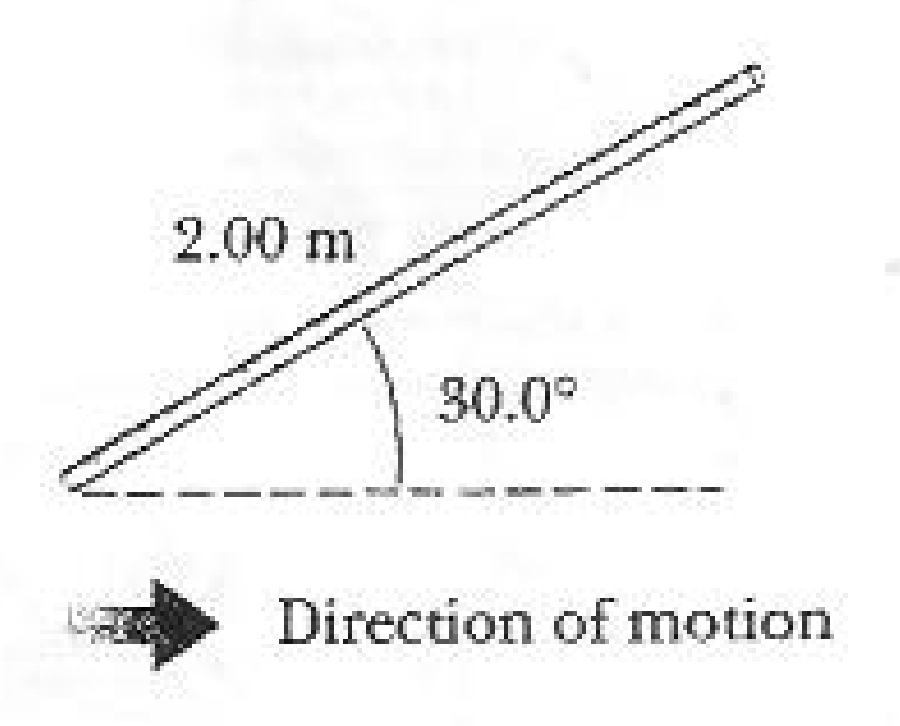
\includegraphics[width=0.7\linewidth]{spho_book_TYS_images/2011q10.png}
	\caption{Relativistic Rod}
\end{figure}
(i) Determine the proper length of the rod. [3] \\
(ii) What is the orientation angle in the proper frame? [3] \\


\end{document}
